\documentclass[12pt,a4paper]{article}
\usepackage[utf8]{inputenc}
\usepackage[T1]{fontenc}
\usepackage[ngerman]{babel}
\usepackage{graphicx}
\usepackage{geometry}
\usepackage{hyperref}
\usepackage{fancyhdr}
\usepackage{xcolor}

\geometry{margin=2.5cm}
\pagestyle{fancy}
\fancyhf{}
\rhead{Mensa Web-App}
\lhead{Allgemeine Kundendokumentation}
\cfoot{\thepage}

\title{\textbf{Benutzerhandbuch \& Kundendokumentation} \\ \Large Mensa Web-Applikation}
\author{Küchenteam \& IT-Administration}
\date{\today}

\begin{document}

\maketitle

\section{Überblick}
Willkommen zur neuen Mensa Web-App! Dieses System wurde entwickelt, um Ihnen den täglichen Speiseplan übersichtlich darzustellen und Ihnen die Möglichkeit zu geben, aktiv an der Gestaltung des Menüs mitzuwirken.

Die Web-App ist für die Nutzung auf PCs, Tablets und Smartphones (Android \& iOS) gleichermaßen optimiert.

\section{Navigation und Bedienung}
Die Anwendung nutzt ein modernes Tab-System. Sie können zwischen den Hauptfunktionen wechseln, ohne dass die Seite komplett neu geladen werden muss:
\begin{itemize}
    \item \textbf{Speiseplan:} Die aktuelle Wochenübersicht.
    \item \textbf{Wochen-Wahl:} Die Abstimmung für das Menü der kommenden Woche.
    \item \textbf{Vorschlag / Umfrage:} Einreichen und Bewerten von Wunschgerichten.
    \item \textbf{Kontakt:} Direkter Draht zum Küchenteam.
    \item \textbf{Login:} Bereich für Administratoren.
\end{itemize}

\section{Der Speiseplan}
Auf der Startseite finden Sie den aktuellen Plan.
\begin{enumerate}
    \item \textbf{Kategorien:} Die Gerichte sind farblich nach \textbf{Vollkost}, \textbf{Leichte Vollkost} und \textbf{Vegetarisch} unterteilt.
    \item \textbf{Heute-Markierung:} Der aktuelle Wochentag wird hervorgehoben und auf Mobilgeräten automatisch in den Fokus gerückt.
    \item \textbf{Zusatzstoffe:} Unter dem Plan finden Sie einen Link zu einer detaillierten Liste aller Allergene und Zusatzstoffe.
\end{enumerate}

\section{Teilnahme an Abstimmungen}
In der Sektion \textbf{"Wochen-Wahl"} können Sie für die Gerichte der nächsten Woche stimmen:
\begin{itemize}
    \item Wählen Sie pro Tag Ihr bevorzugtes Gericht aus.
    \item Klicken Sie am Ende der Liste auf "Abstimmen".
    \item \textit{Hinweis:} Um faire Ergebnisse zu gewährleisten, bitten wir darum, nur einmal pro Woche abzustimmen.
\end{itemize}

\section{Wunschspeisen und Spezial-Umfragen}
Ein besonderes Highlight ist das Mitbestimmungsrecht:
\begin{itemize}
    \item \textbf{Vorschlag einreichen:} Senden Sie uns Ihre Ideen für neue Gerichte.
    \item \textbf{Bewertung:} Stimmen Sie für die Vorschläge anderer Nutzer. Die beliebtesten Gerichte werden regelmäßig in den echten Speiseplan übernommen.
    \item \textbf{Fortschrittsbalken:} In den Ergebnissen sehen Sie direkt, wie viel Prozent der Stimmen ein Gericht erhalten hat.
\end{itemize}

\section{Kontakt und Ticket-System}
Wenn Sie eine Frage oder Anregung haben, nutzen Sie das Kontaktformular.
\begin{itemize}
    \item \textbf{Nachricht senden:} Geben Sie Ihr Thema und Ihren Text ein.
    \item \textbf{Ticket anfordern:} Wenn Sie eine Antwort von uns wünschen, kreuzen Sie "Antwort gewünscht" an.
    \item \textbf{Sicherheit:} Sie erhalten eine \textbf{Ticket-ID} und ein \textbf{Geheimwort}. Bitte speichern Sie beides gut ab!
    \item \textbf{Antwort abrufen:} Unter dem Tab "Antwort abrufen" können Sie mit Ihren Zugangsdaten schauen, ob wir bereits geantwortet haben.
\end{itemize}

\section{Leitfaden für Administratoren (Küchenpersonal)}
Nach dem Login im Dashboard stehen Ihnen erweiterte Funktionen zur Verfügung:
\begin{itemize}
    \item \textbf{Auswertung:} Sehen Sie sofort, welche Gerichte für die nächste Woche gewonnen haben.
    \item \textbf{Speisenverwaltung:} Hinzufügen, Bearbeiten oder Löschen von Gerichten in der Datenbank.
    \item \textbf{Wochenplan-Pflege:} Erstellen Sie den Plan für die kommende Woche mit wenigen Klicks.
    \item \textbf{Umfrage-Management:} Starten Sie neue Umfragen oder aktivieren Sie das Wunschspeisen-Modul.
    \item \textbf{Ticket-Bearbeitung:} Antworten Sie auf Anfragen von Nutzern direkt im System.
\end{itemize}

\section{Hilfe und Support}
Sollten technische Probleme auftreten, wenden Sie sich bitte an die IT-Administration oder nutzen Sie das Kontaktformular mit dem Betreff "Technischer Support".

\appendix
\section{Anhang: Visuelle Übersicht}
In diesem Anhang finden Sie Screenshots der wichtigsten Bereiche der Applikation zur Verdeutlichung der Funktionen.

\newpage
\subsection{Startseite: Der Speiseplan}
Die moderne, tabellarische Ansicht des Speiseplans mit Farbcodes für die verschiedenen Kategorien.
\begin{figure}[h]
    \centering
    \fbox{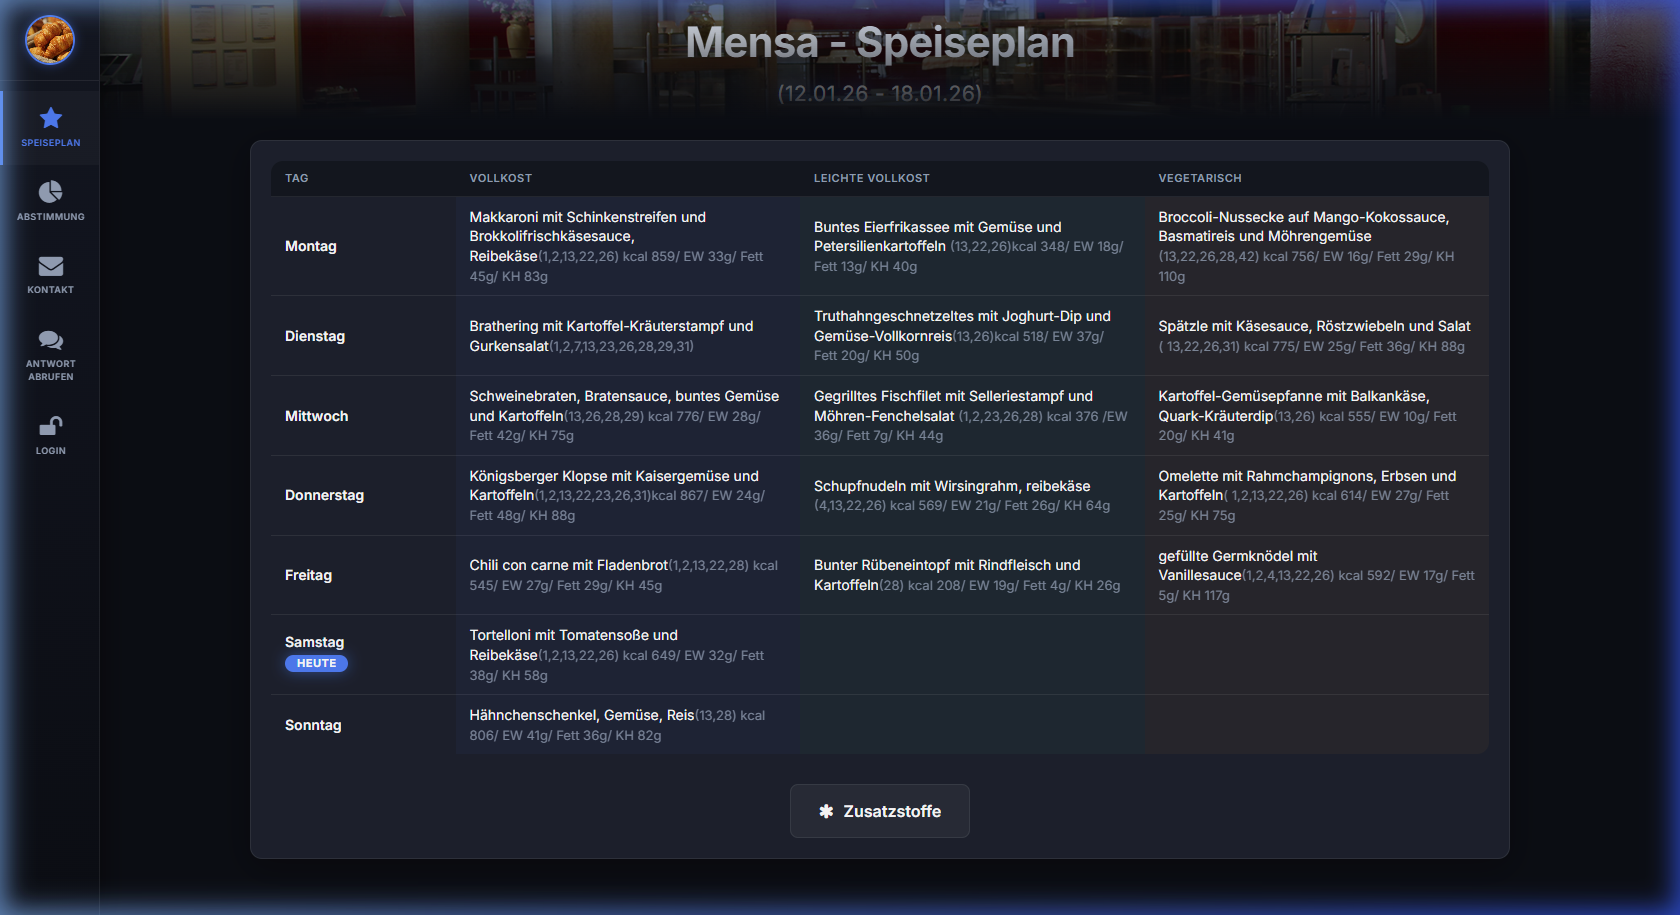
\includegraphics[width=0.8\textwidth]{images/speiseplan.png}}
    \caption{Der interaktive Speiseplan auf der Startseite.}
\end{figure}

\subsection{Wochen-Wahl (Abstimmung)}
Formular zur Auswahl der Gerichte für die kommende Woche.
\begin{figure}[h]
    \centering
    \fbox{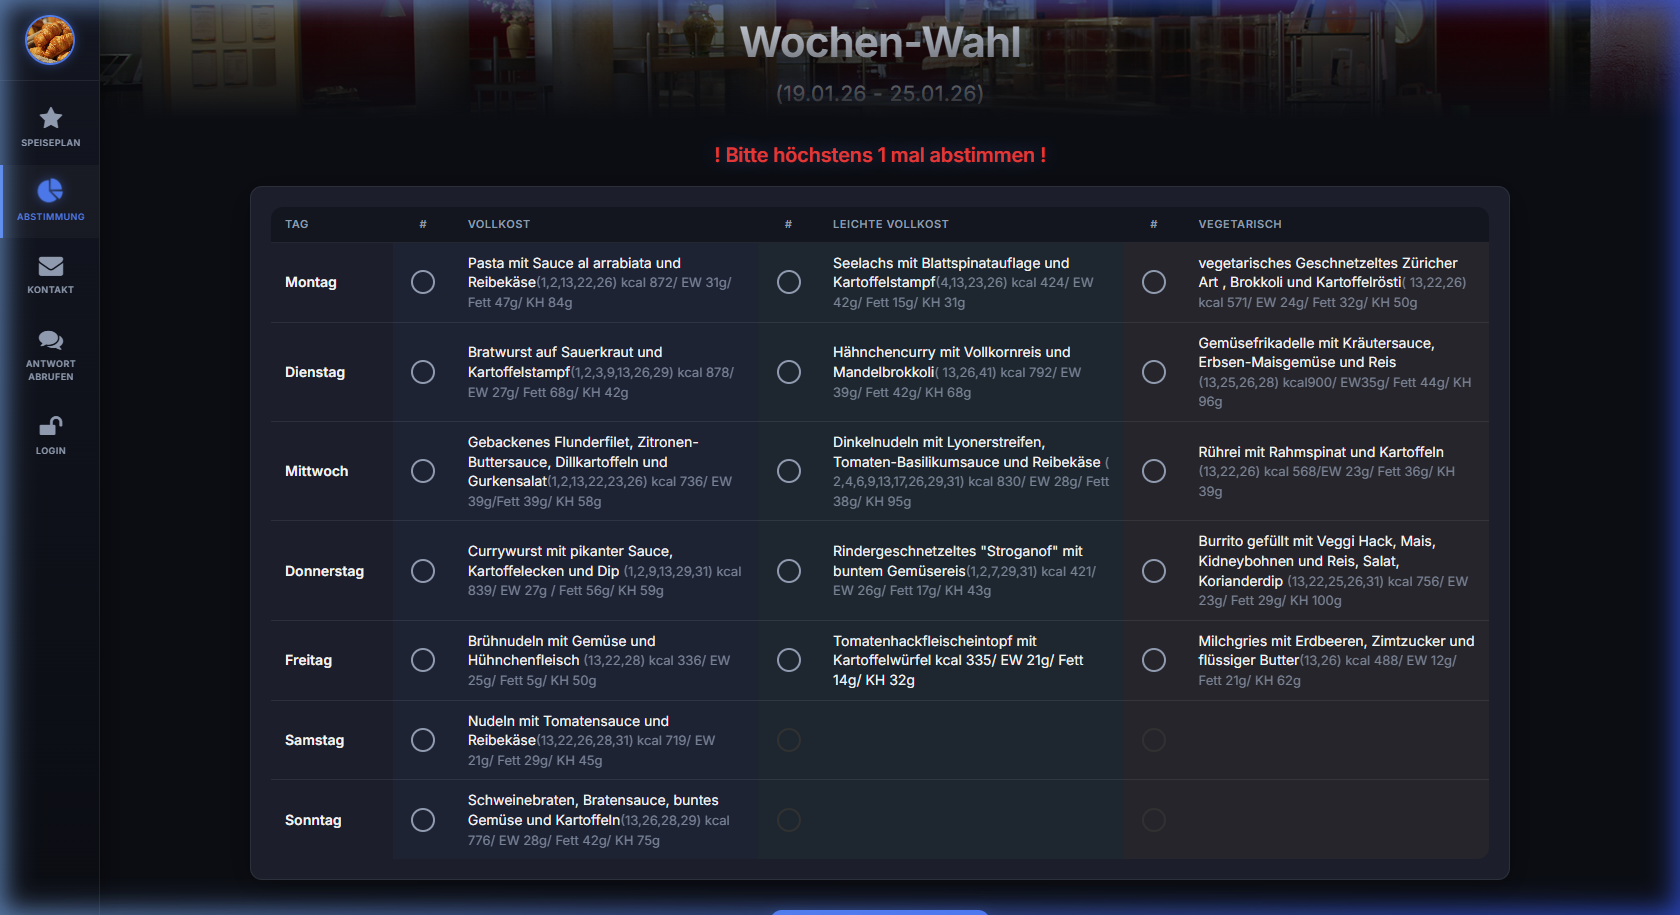
\includegraphics[width=0.8\textwidth]{images/wahl.png}}
    \caption{Das Abstimmungsmodul für Nutzer.}
\end{figure}

\newpage
\subsection{Umfragen \& Wunschspeisen}
Darstellung der Ergebnisse mit dynamischen Fortschrittsbalken.
\begin{figure}[h]
    \centering
    \fbox{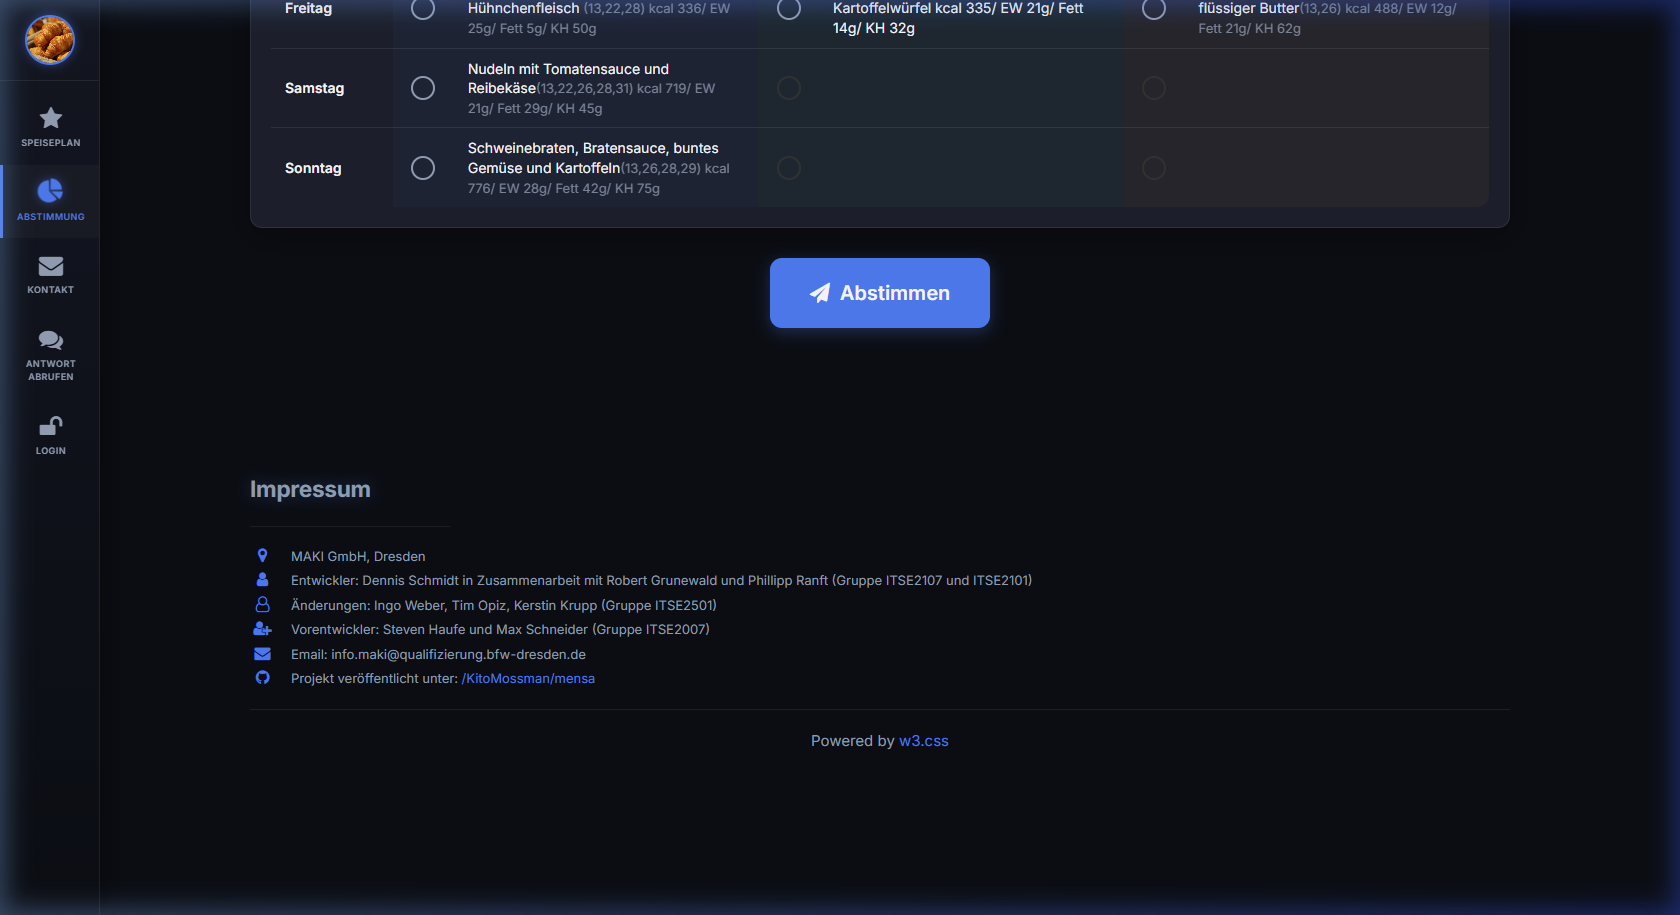
\includegraphics[width=0.8\textwidth]{images/umfrage_ergebnis.png}}
    \caption{Ergebnisauswertung mit visuellen Indikatoren.}
\end{figure}

\subsection{Kontakt \& Ticket-Status}
Einfache Kommunikation mit integrierter Ticket-Abfrage.
\begin{figure}[h]
    \centering
    \fbox{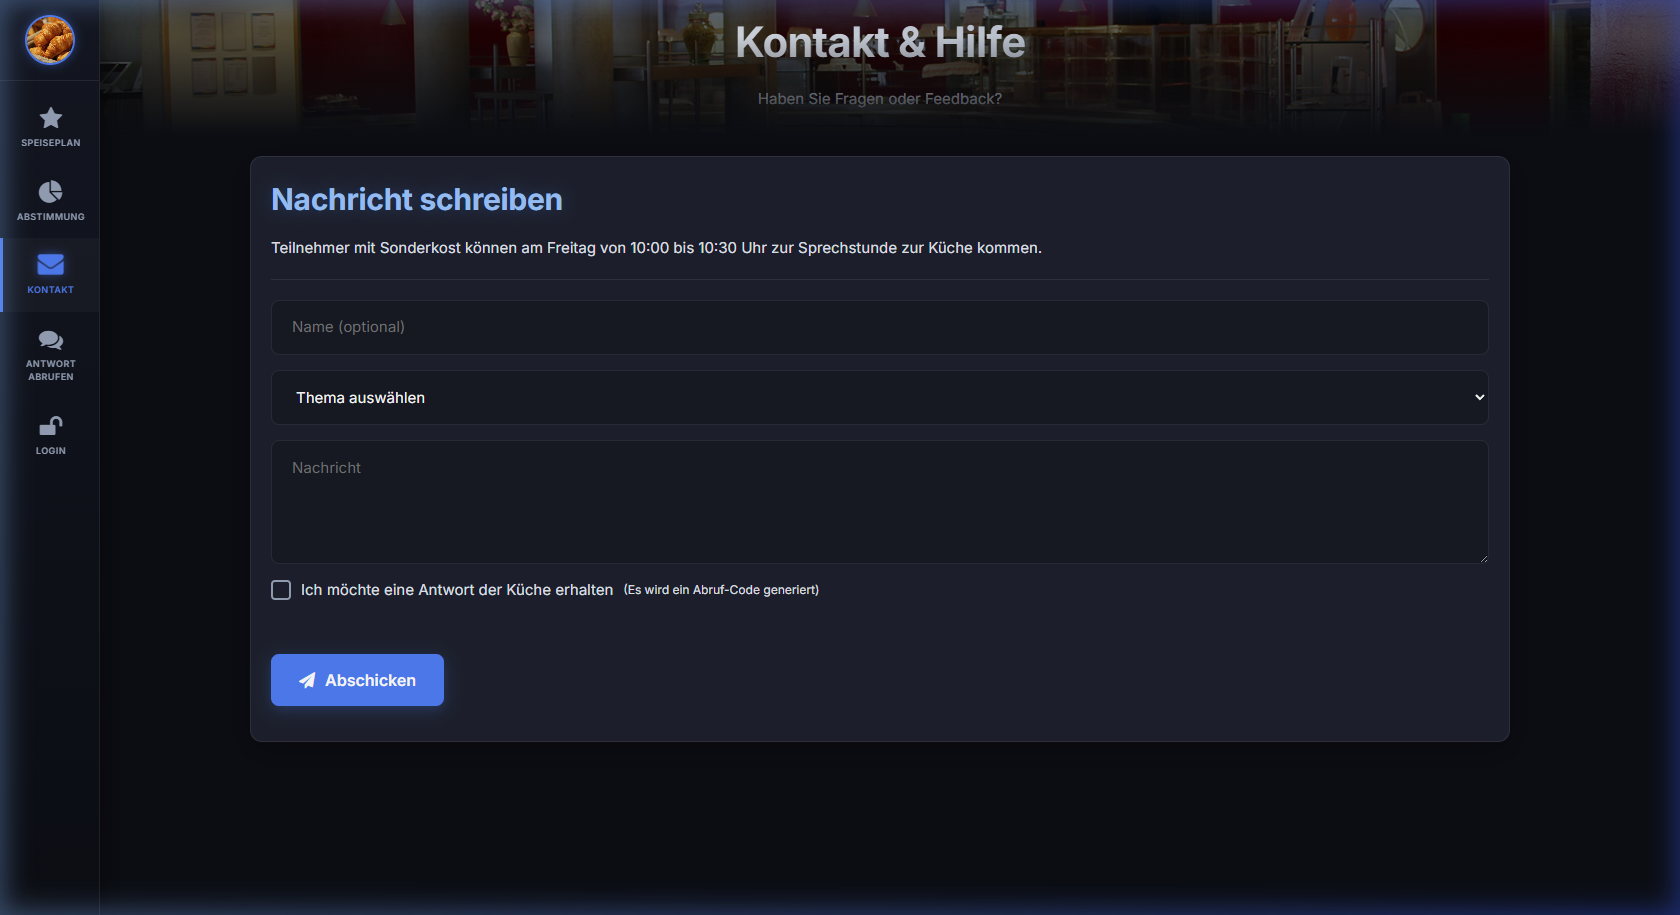
\includegraphics[width=0.8\textwidth]{images/kontakt.png}}
    \caption{Kontaktformular mit Ticket-Generierung.}
\end{figure}

\newpage
\subsection{Admin Dashboard (Küche)}
Die zentrale Verwaltungsoberfläche für das Küchenpersonal.
\begin{figure}[h]
    \centering
    \fbox{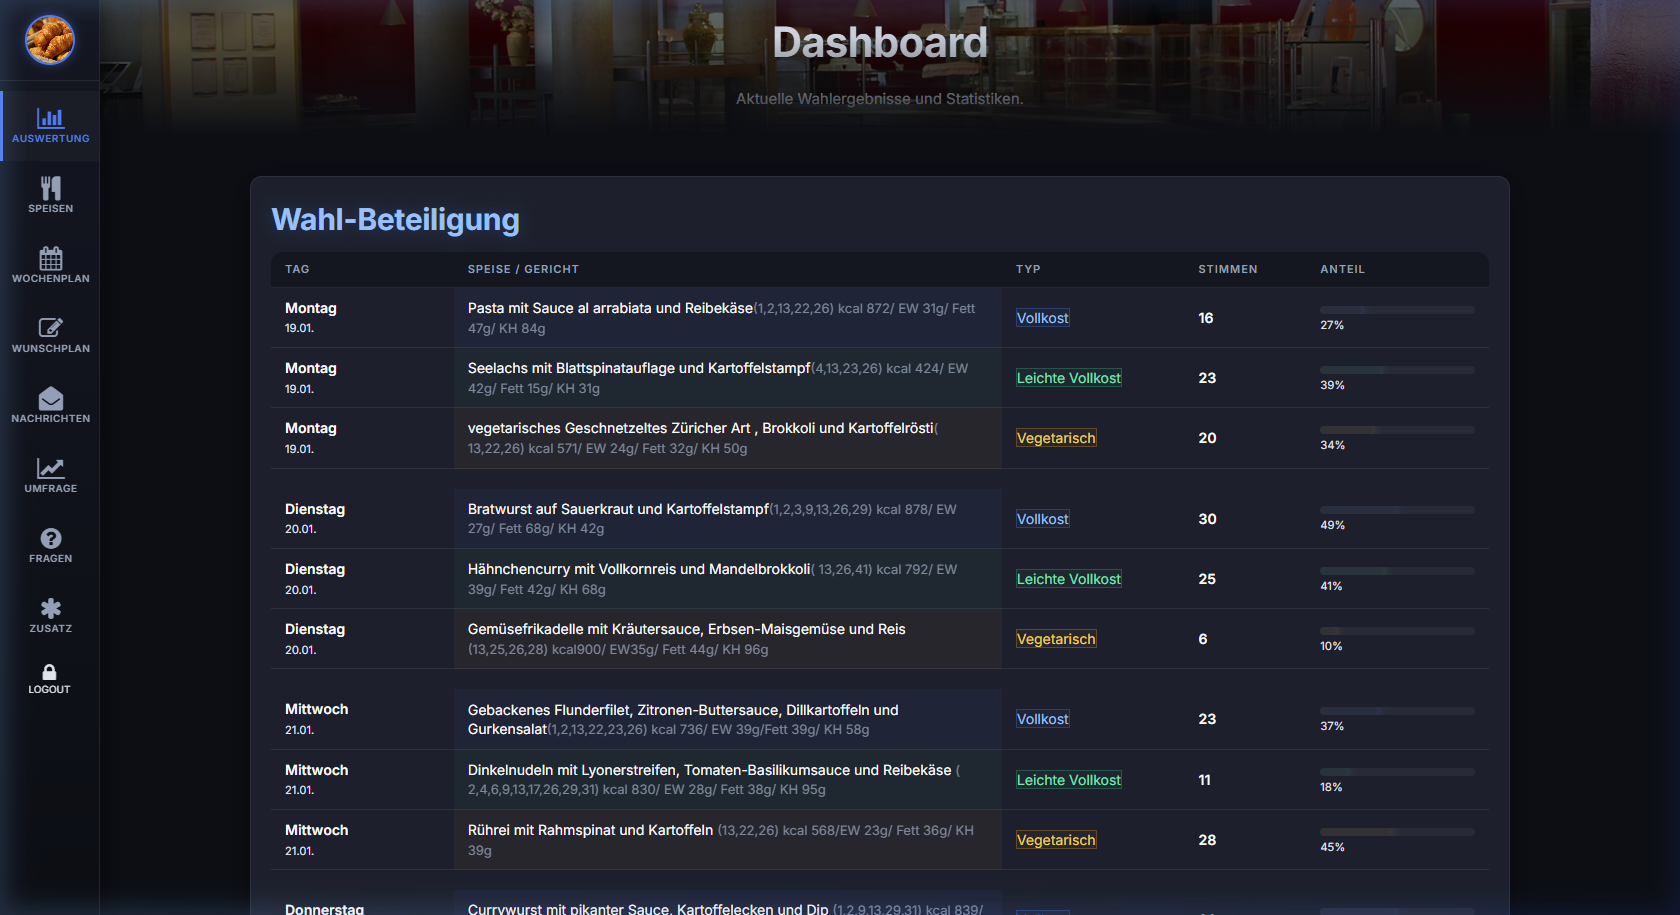
\includegraphics[width=0.8\textwidth]{images/admin_dashboard.png}}
    \caption{Übersicht der Wahlergebnisse im Administrationsbereich.}
\end{figure}

\subsection{Nachrichtenverwaltung}
Bearbeitung eingehender Anfragen und Tickets.
\begin{figure}[h]
    \centering
    \fbox{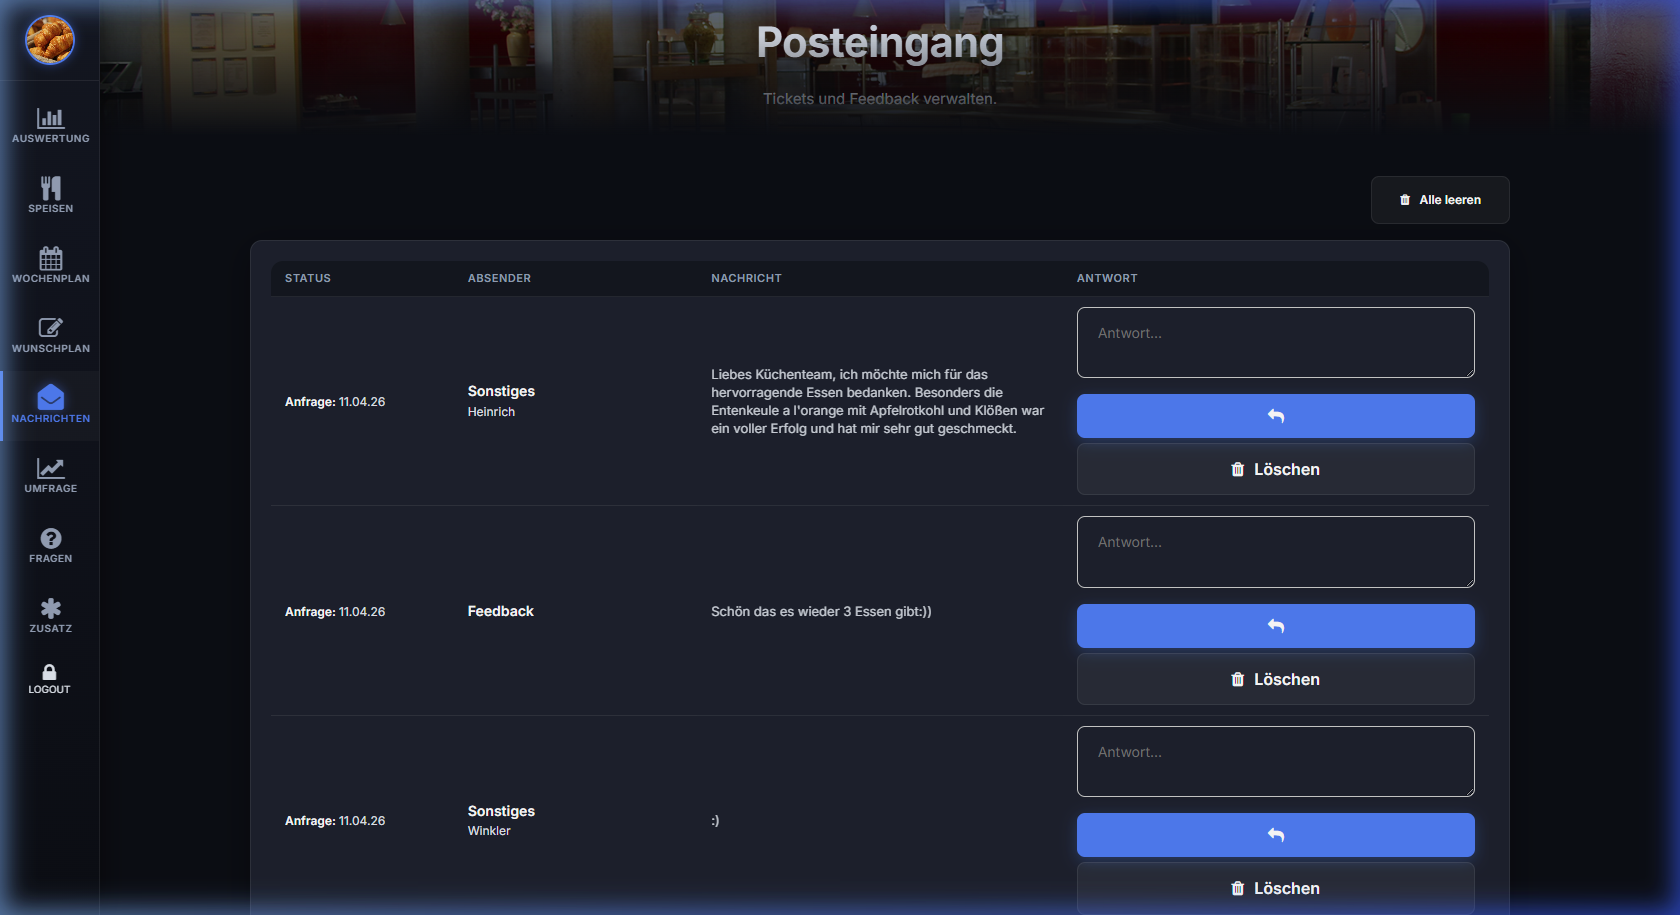
\includegraphics[width=0.8\textwidth]{images/admin_nachrichten.png}}
    \caption{Posteingang für Nutzer-Anfragen im Dashboard.}
\end{figure}

\end{document}
